\documentclass[aspectratio=169,dvipsnames]{beamer}
\usetheme{Pittsburgh}
\usepackage[utf8]{inputenc}
\usepackage{amsmath}
\usepackage{amsfonts}
\usepackage{amssymb}
\usepackage{graphicx}
\usepackage{multicol}
\usepackage{wrapfig}
\usepackage{hyperref}
\usepackage{censor}

\usepackage{tikz}
\usetikzlibrary{shapes,arrows,chains}

\author{Jonas Betzendahl}
\title{Digital Self-Defense}

\beamertemplatenavigationsymbolsempty 
\setbeamertemplate{footline}[frame number]

%src: https://tex.stackexchange.com/questions/34921/how-to-overlap-images-in-a-beamer-slide
\def\Put(#1,#2)#3{\leavevmode\makebox(0,0){\put(#1,#2){#3}}}

%https://tex.stackexchange.com/questions/70448/dont-count-backup-slides
\newcommand{\backupbegin}{
   \newcounter{finalframe}
   \setcounter{finalframe}{\value{framenumber}}
}
\newcommand{\backupend}{
   \setcounter{framenumber}{\value{finalframe}}
}

\begin{document}

%------------------------------------------------------------------------------------
\section{Introduction}

\begin{frame}
\begin{center}
\vfill
\huge Digital Self-Defense
\normalsize 
\smallskip
\smallskip

Levelling up your defense in a world\\ that is levelling up its offense.
\bigskip\bigskip

\large Jonas Betzendahl, M.Sc.\\
2019 -- 12 -- 06
\bigskip\bigskip

\href{https://twitter.com/lambdatotoro}{\includegraphics[scale=0.125]{images/twitter_logo.png}}
\href{https://chaos.social/@lambdatotoro}{\includegraphics[scale=0.125]{images/mastodon_logo.png}}
\href{https://github.com/lambdaTotoro}{\includegraphics[scale=0.125]{images/github_logo.png}}
\href{https://whispeer.de/en/user/jbetzend}{\includegraphics[scale=0.125]{images/whispeer_logo.png}}

\texttt{@lambdaTotoro (@chaos.social)}
\end{center}
\end{frame}

\begin{frame}
\frametitle{Who am I?}
\begin{minipage}{0.6\textwidth}
\Large Jonas Betzendahl\normalsize\\
\texttt{lambdatotoro@posteo.de}
\bigskip

\begin{itemize}
\item Bielefeld University\\Cognitive Informatics + Intelligent Systems
\item Now @ FAU Erlangen-Nürnberg\\Knowledge Representation and Management
\item Love for teaching and science communication
\item Favourite topics: misconceptions about and risks of technology.
\end{itemize}

\end{minipage}%
\begin{minipage}{0.4\textwidth}
\begin{center}
\includegraphics[scale=0.15,keepaspectratio]{images/pigeon_jonas}
\end{center}
\end{minipage}
\end{frame}

\begin{frame}
\frametitle{Who are you?}
\begin{minipage}{0.4\textwidth}
\begin{center}
\includegraphics[scale=0.4]{images/smartphone} 
\end{center}
\end{minipage}%
\begin{minipage}{0.6\textwidth}
I have no idea who you are! But I'm making a few assumptions. 
In all likelihood, you \dots
\medskip

\begin{itemize}
\pause\item\emph{don't} necessarily have a degree in computer science or a related field.
\pause\item\emph{do} regularly interact with computers, probably both professionally and privately.
\end{itemize}
\end{minipage}
\end{frame}

\begin{frame}[fragile]
\frametitle{What is the problem?}

Before we can talk about digital \emph{self-defense}, we need an idea about digital \emph{violence}.
\pause\bigskip

\begin{verbatim}
Digital violence is all violence that uses digital tools (computers,
phones, apps,...), digital media (video, email,...) or occurs within
online spaces.
\end{verbatim}
\pause
\begin{verbatim}
We believe that usually, digital violence does not happen in
isolation from "analogue violence" but often forms an addition to
or a continuation of preexisting violent contexts.

\end{verbatim}
\end{frame}

\begin{frame}
\frametitle{What is \emph{not} the solution?}

A common problem that is making things worse:
\bigskip

\begin{center}
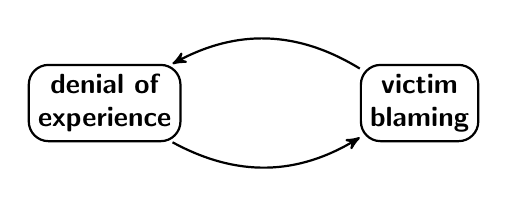
\begin{tikzpicture}[->,>=stealth',auto,node distance=4cm, 
  thick,main node/.style={clip, align=center, rounded corners=0.25cm,draw,font=\sffamily\bfseries}]

  \node[main node] (1) {denial of\\ experience};
  \node[main node] (2) [right of=1] {victim\\ blaming};

  \path[every node/.style={font=\sffamily\small}]
    (1) edge[bend right] node [right] {} (2)
    (2) edge[bend right] node [left] {} (1);
\end{tikzpicture}
\end{center}
\pause\bigskip

\begin{itemize}
\item ``That's not that bad!'', ``It's not harassment if you can just log off!'', \dots
\item ``Don't feed the troll!'', ``Don't take nudes!'', ``Don't be online!'', \dots
\end{itemize}
\end{frame}

\begin{frame}
\frametitle{What \emph{is} the solution?}
\begin{center}
\Large
Sometimes, sunlight is the best disinfectant.
\end{center}
\normalsize\bigskip

Many attacks in the digital realm can only work if the victim doesn't know about them, isn't sensitised to them or reacts wrongly to them.
\medskip\pause

This workshop is to give you an overview of some of the most important attacks and what to do about them.
\end{frame}

\begin{frame}
\frametitle{What is this workshop?}

\begin{minipage}{0.5\textwidth}
I will be giving input, but this is \emph{not}\\ a lecture.
\bigskip

I'd rather have a conversation than\\ finish all my slides.
\bigskip

Please ask questions immediately, do\\ feel free to interrupt at any point.
\end{minipage}%
\begin{minipage}{0.5\textwidth}
\begin{center}
\includegraphics[scale=0.6,keepaspectratio]{images/conversation.png} 
\end{center}
\end{minipage}
\end{frame}

%------------------------------------------------------------------------------------

\section{Technical Attacks}
\begin{frame}
\begin{center}
\huge Technical Attacks\normalsize
\end{center}
\end{frame}

\subsection{Passwords}

\subsubsection{Secure Passwords}

\begin{frame}
\frametitle{Secure Passwords}
\begin{minipage}{0.5\textwidth}
Passwords are usually the first and most important barrier between our accounts and those that would take them.
\bigskip

Good passwords should resist both \emph{dictionary} and \emph{brute-force}
and hence be\dots 
\medskip

\begin{itemize}
\item\dots uncommon, ideally unique.
\item\dots not too short ($\geq 12$ characters).
\item\dots high-entropy\\ (contain letters, numbers, specials).
\end{itemize}
\end{minipage}%
\begin{minipage}{0.5\textwidth}
\begin{center}
\includegraphics[scale=0.6]{images/hacker.png} 
\end{center}
\end{minipage}
\end{frame}

\setbeamercolor{background canvas}{bg=Apricot}

\begin{frame}
\frametitle{Passwords (Quiz)}

Which of these is the ``worst'' (cum kilo salis) way to do passwords?
\bigskip

\begin{itemize}
\item Using many different weak passwords.
\item Using the same strong password on all sites.
\item Using many different strong passwords,\\ but write them down next to your computer.
\end{itemize}

\end{frame}

\begin{frame}
\frametitle{Passwords (Quiz)}

Which of these is the ``worst'' (cum kilo salis) way to do passwords?
\bigskip

\begin{itemize}
\item \textcolor{ForestGreen}{Using many different weak passwords.}
\item \textcolor{ForestGreen}{Using the same strong password on all sites.}
\item \textcolor{Red}{Using many different strong passwords,\\ but write them down next to your computer.}
\end{itemize}

\end{frame}

\setbeamercolor{background canvas}{bg=white}

\begin{frame}
\frametitle{Common Passwords}
Any of these ring a bell? The most common passwords\dots
\bigskip\bigskip

\begin{minipage}{0.5\textwidth}
\begin{center}
\dots in Germany:
\end{center}
\bigskip

\begin{minipage}{0.5\textwidth}
\begin{itemize}
\item 123456
\item 12345
\item 123456789
\item ficken
\item 12345678
\end{itemize}
\end{minipage}%
\begin{minipage}{0.5\textwidth}
\begin{itemize}
\item hallo123
\item hallo
\item 123
\item passwort
\item master
\end{itemize}
\end{minipage}
\end{minipage}%
\begin{minipage}{0.5\textwidth}
\begin{center}
\dots worldwide
\end{center}
\bigskip

\begin{minipage}{0.5\textwidth}
\begin{itemize}
\item 123456
\item 123456789
\item qwerty
\item password
\item 111111
\end{itemize}
\end{minipage}%
\begin{minipage}{0.5\textwidth}
\begin{itemize}
\item 12345678
\item abc123
\item 1234567
\item password1
\item 12345
\end{itemize}
\end{minipage}
\end{minipage}

\end{frame}

\begin{frame}
\frametitle{Password Reuse}
\begin{center}
\includegraphics[scale=0.43]{images/password_reuse.png} 
\end{center}
\end{frame}

\begin{frame}[fragile]
\frametitle{Passwords from Stories}

One way of generating passwords that are easy for humans to remember but hard for computers to guess: Generate a sentence you associate with the website an use all beginning letters plus numbers and punctuation.
\pause\bigskip\bigskip

\emph{Example Amazon Password:}
\begin{center}
\large
``\textbf{I} \textbf{w}ish \textbf{J}eff \textbf{B}ezos \textbf{w}ould \textbf{d}o
\textbf{s}omething \textbf{u}seful \textbf{w}ith \textbf{h}is \textbf{110} \textbf{B}illion \textbf{Dollars!}''
\bigskip

becomes
\bigskip

IwJBwdsuwh110B\$!
\end{center}
\begin{flushright}
\small
(crackable in 39555681645472620 years)
\end{flushright}

\normalsize
\end{frame}

\subsubsection{Password Managers}

\begin{frame}
\frametitle{Password Managers}
Another way of avoiding password reuse while still using strong passwords are \emph{password managers}. These are software secured with one master password that remember all your other passwords. They also can generate secure passwords:
\pause\bigskip

Like this one:
\begin{center}
\texttt{1kgaV|FKkYC?q=p\$1WxG9vSL;932Z.h\&}
\end{center}
\pause\bigskip

There are many options (commercial and open source) for Windows, Mac, Linux, Android, iOS, \dots that can also sync (manually or via cloud) across devices. Also consider analogue ones.
\end{frame}

\subsubsection{Security Questions}

\begin{frame}
\frametitle{Security Questions}
\end{frame}


\subsubsection{Phone Security}

\setbeamercolor{background canvas}{bg=Apricot}

\begin{frame}
\frametitle{Smartphone Security (Quiz)}

Which of these is the safest way of locking your phone?
\medskip

\begin{itemize}
\item A six-digit PIN
\item A six-point swipe pattern
\item Your fingerprint / face as a biometric pattern
\end{itemize}

\end{frame}

\begin{frame}
\frametitle{Smartphone Security (Quiz)}

Which of these is the safest way of locking your phone?
\medskip

\begin{itemize}
\item \textcolor{ForestGreen}{A six-digit PIN}
\item \textcolor{Red}{A six-point swipe pattern}
\item \textcolor{Red}{Your fingerprint / face as a biometric pattern}
\end{itemize}

\end{frame}

\setbeamercolor{background canvas}{bg=white}

\begin{frame}
\frametitle{Swipe Patterns}

\begin{minipage}{0.5\textwidth}
Swipe patterns are not as safe as a pin number of the same length.
\bigskip

Studies have shown they are easier to gleam ``over the shoulder'' and can sometimes also be reconstructed from smudge marks.
\end{minipage}%
\begin{minipage}{0.5\textwidth}
\begin{center}
\includegraphics[scale=0.3]{images/swipe_unlock.jpg} 
\end{center}
\end{minipage}

\end{frame}

\begin{frame}
\frametitle{Biometrics}

\begin{minipage}{0.5\textwidth}
\begin{center}
\includegraphics[width=0.95\textwidth, keepaspectratio]{images/hirevue.jpeg}
\end{center}
\end{minipage}\quad
\begin{minipage}{0.45\textwidth}
Biometrics (such as fingerprints, facial recognition, \dots) are very convenient!
\medskip

But they are not good passwords! For example, they can't be \dots

\begin{itemize}
\pause\item changed or reset,
\pause\item ``forgotten'',
\pause\item fake-proofed
\end{itemize}
\end{minipage}

\pause\bigskip
\begin{center}
\Large
Biometrics are better thought of as \emph{user names}, not \emph{passwords}!
\end{center}
\end{frame}

\subsubsection{Leaks}

\begin{frame}
\frametitle{Leaks \& Data Breaches}
\end{frame}

\setbeamercolor{background canvas}{bg=Apricot}

\begin{frame}
\frametitle{Have I been pwned?}

Take a few minutes and visit one of these leak detection services:

\begin{itemize}
\item\url{https://haveibeenpwned.com/}
\item\url{https://sec.hpi.de/ilc/}
\end{itemize}
\bigskip

Enter your own email to see if any of your accounts have been compromised in big leaks in the past. If they have, consider changing your password(s) soon.
\bigskip\bigskip

If you feel uncomfortable using your own email address, you can use one of mine:
\begin{center}
\texttt{jonas.betzendahl@gmail.com}
\end{center}

\end{frame}

\setbeamercolor{background canvas}{bg=white}

\subsection{Malware}

\subsubsection{Keyloggers, Trojans, Viruses}

\begin{frame}
\frametitle{Keyloggers, Trojans, Viruses}
\end{frame}

\subsubsection{Stalkerware}

\begin{frame}
\frametitle{Stalker- \& Spouseware}

A growing phenomenon in recent years, Stalkerware is monitoring software (often marketed as ``catching cheating spouses'' or ``kid surveillance'') that is installed on the victims phone by an attacker the victim knows.
\bigskip

These kinds of malware can\dots

\begin{itemize}
\item\dots forward and record all texts, messages, calls.
\item\dots make location data available.
\item\dots record video and audio at all times.
\end{itemize}

\end{frame}

\begin{frame}
\frametitle{How to spot Stalkerware}

There is \emph{no} guaranteed way of confirming that you do not have Stalkerware on your phone. However, there are a few common warning signs:
\bigskip

\begin{itemize}
\pause\item High battery usage
\pause\item Apps, even innocuous-seeming ones, that you don't remember installing.
\pause\item Apps from unrecognised sources\\ \emph{Android:} Settings $\Rightarrow$ Security $\Rightarrow$ Allow unknown sources\\ \emph{Apple:} Jailbroken Phone
\pause\item People in your life that seem to know things they should have no way of knowing.
\end{itemize}
\pause\bigskip

It's very difficult to get rid of this malware because it is designed to be resilient and avoid detection. The ultima ratio is a factory reset.
\end{frame}


\begin{frame}
\frametitle{CryptoLockers}
\begin{minipage}{0.6\textwidth}
\begin{center}
\includegraphics[scale=0.2]{images/cryptolocker.jpg} 
\end{center}
\end{minipage}%
\begin{minipage}{0.4\textwidth}
CryptoLockers / Ransomware encrypts all files on your computer it can find and asks for money.
\pause\medskip

\emph{Don't Panic!} Research the malware, maybe there's a fix.
\pause\medskip

Prevention is the best medicine. Keep your systems up-to-date and have recent external backups.
\end{minipage}
\end{frame}

\subsubsection{Anti-virus Software}

\begin{frame}
\frametitle{Anti-Virus}
\end{frame}

\begin{frame}
\frametitle{Not just for Desktops}
\end{frame}

\subsection{VPNs}

\begin{frame}
\frametitle{VPNs}
\end{frame}

\begin{frame}
\frametitle{VPN Advertisement Claims:}

\begin{itemize}
\item \textbf{``Everytime you connect to public Wi-Fi, you risk data theft!''}
\pause \item \textbf{``This VPN uses military-grade encryption!''}\\
True, but meaningless.
\end{itemize}


\pause
\begin{center}
\emph{Recommended Watch: Tom Scott's ``This Video Is Sponsored By \censor{Nord}VPN''}
\end{center}
\end{frame}

%------------------------------------------------------------------------------------

\section{Social Attacks}
\begin{frame}
\begin{center}
\huge Social Attacks
\end{center}
\end{frame}

\begin{frame}
\frametitle{No setup gives perfect security!}
\begin{center}
\includegraphics[height=0.65\textheight,keepaspectratio]{images/security.png} 
\end{center}
\end{frame}

\begin{frame}
\frametitle{How it works\dots}
\begin{minipage}[t]{0.49\textwidth}
\begin{center}
\vspace*{-15pt}
\includegraphics[width=\textwidth,keepaspectratio]{images/hackerman-1}
\end{center}
\end{minipage}
\begin{minipage}[t]{0.49\textwidth}
\begin{center}
\vspace*{15pt}
\includegraphics[width=\textwidth,keepaspectratio]{images/hackerman-2}
\end{center}
\end{minipage}
\end{frame}

\subsection{Phishing}

\begin{frame}
\frametitle{Phishing (1)}

\end{frame}

\begin{frame}
\frametitle{Phishing (2)}
\begin{center}
\includegraphics[scale=0.45]{images/phishing.png} 
\end{center}
\end{frame}

\begin{frame}
\frametitle{Phishing (3)}
\begin{center}
\includegraphics[scale=0.375]{images/phishing_gov} 
\end{center}
\end{frame}

\begin{frame}
\frametitle{Phishing (4)}
\begin{center}
\includegraphics[scale=0.175]{images/phishing_apple.png} 
\end{center}
\end{frame}

\begin{frame}
\frametitle{Phishing (5)}
\begin{center}
\includegraphics[scale=0.375]{images/bait} 
\end{center}
\end{frame}

\subsection{Social Engineering}

\begin{frame}
\frametitle{Social Engineering}
\end{frame}

\setbeamercolor{background canvas}{bg=Apricot}

\begin{frame}
\frametitle{Social Engineers}

Coordinate with one or more partners from around the room, exchange names and -- given that you have their consent -- with the search engine of your choice, try and find out some personal information about them or yourself that could be used to either find more information or wrongly authenticate yourself as them in front of third parties.
\bigskip

If any of you feel uncomfortable with this exercise, that is absolutely okay. Nobody has to participate if they do not wish it. If your group has no volunteers, take me instead (my full name, again, is ``Jonas Betzendahl'').

\end{frame}

\setbeamercolor{background canvas}{bg=white}

%------------------------------------------------------------------------------------

\section{Miscellaneous}

\begin{frame}
\begin{center}
\huge Miscellaneous
\end{center}
\end{frame}

\subsection{IoT}

\begin{frame}
\frametitle{Internet of Things}

\begin{minipage}{0.4\textwidth}
\begin{center}
\includegraphics[scale=0.25,keepaspectratio]{images/alexa}
\end{center}
\end{minipage}%
\begin{minipage}{0.6\textwidth}
Over the past few years, more and more internet-enabled devices (voice assistants, doors, toasters, even dolls!) have moved into ``smart homes''.
\pause\medskip

The companies behind these products often have poor standards of operational security and data safety. 
\pause\medskip

There is little to say besides ``Don't get one.'', but if you do, research the device beforehand and make sure that firmware is up-to-date and default credentials are changed.
\end{minipage}
\end{frame}

\subsection{Secure Messaging}

\begin{frame}
\frametitle{Secure Messaging Apps (1)}
\begin{center}
\includegraphics[scale=0.5]{images/signal_whatsapp_telegram.png} 
\end{center}
\end{frame}

\begin{frame}
\frametitle{Secure Messaging Apps (2)}
\begin{center}
More detailed overview: \url{https://www.securemessagingapps.com/}
\bigskip

\includegraphics[scale=0.25, keepaspectratio]{images/secure_messengers_comparison.png} 
\end{center}
\end{frame}

\subsection{Multi-Factor Authentication}

\begin{frame}
\frametitle{2FA}
\end{frame}

\subsection{Fake News}

\begin{frame}
\frametitle{Fake News}


\begin{itemize}
\item English: \url{https://www.snopes.com}
\item German: \url{https://correctiv.org/faktencheck/}
\end{itemize}

\end{frame}

\setbeamercolor{background canvas}{bg=Apricot}

\begin{frame}
\frametitle{Fake News Quiz (1)}
\begin{center}
\includegraphics[scale=0.1]{images/queen} 
\end{center}
\pause
\Put(200,100){\includegraphics[scale=0.3]{images/quiz_correct.png} }
\end{frame}

\begin{frame}
\frametitle{Fake News Quiz (2)}
\begin{center}
\includegraphics[scale=0.3]{images/trump} 
\end{center}
\pause
\Put(200,100){\includegraphics[scale=0.15]{images/quiz_wrong.png} }
\end{frame}

\begin{frame}
\frametitle{Fake News Quiz (3)}
\begin{center}
\includegraphics[scale=0.35]{images/thunberg_antifa.png} 
\end{center}
\pause
\Put(200,100){\includegraphics[scale=0.3]{images/quiz_correct.png} }
\end{frame}

\setbeamercolor{background canvas}{bg=white}

%------------------------------------------------------------------------------------

\section{Conclusion}
\begin{frame}
\begin{center}
\huge Conclusion
\end{center}
\end{frame}

\begin{frame}
\frametitle{Recap}
test
\end{frame}

\begin{frame}
\frametitle{In the long run\dots}
\begin{center}
\includegraphics[scale=0.25]{images/kipping.png}
\bigskip

\Large
Learn \& Teach
\end{center}
\end{frame}

\begin{frame}
\frametitle{Things you can do this weekend:}

The best things to keep in mind are the things that you can do soon:
\bigskip

\begin{itemize}
\pause\item\textbf{\dots install newest software updates.}
\pause\item\textbf{\dots install/change lockscreen PIN.}
\pause\item\textbf{\dots get a password manager.}
\pause\item\textbf{\dots check for identity leaks.}
\pause\item\textbf{\dots get a secure (end-to-end) messenger.}
\pause\item\textbf{\dots review apps \& permissions on your phone.}
\pause\item\textbf{\dots install anti-virus software.}\\
\pause\item\textbf{\dots enable 2FA where applicable.}
\end{itemize}
\end{frame}

%------------------------------------------------------------------------------------
\appendix
\backupbegin

\section{End}

\begin{frame}
\frametitle{Resources}

\begin{itemize}
\item \emph{Surveillance Self-Defense} @ EFF, \url{https://ssd.eff.org}
\item \emph{Coalition against Stalkerware}, \url{https://stopstalkerware.org/}
\item \emph{Secure Messaging Apps}, \url{https://www.securemessagingapps.com/}
\item \emph{Identity Leak Checker} @ HPI, \url{https://sec.hpi.de/ilc/}
\item Initiative \emph{Frauen gegen Gewalt}, \url{https://frauen-gegen-gewalt.de}
\end{itemize}

\end{frame}

\begin{frame}
\frametitle{Sources}
\footnotesize

\begin{itemize}
\item Wired, \emph{Don't Rely On an Unlock Pattern To Secure Your Android Phone}: \\
\url{https://www.wired.com/story/android-unlock-pattern-or-pin/}
\item UK Advertisement Regulatory Ruling Re: NordVPN:\\
\url{https://www.asa.org.uk/rulings/tefincom-sa-a19-547668.html}
\item Tom Scott's ``This Video Is Sponsored By \censor{Nord}VPN'':\\
\url{https://www.youtube.com/watch?v=WVDQEoe6ZWY}
\item ExtremeTech's \emph{``Most Android Anti-Malware Apps Don’t Offer Any Protection''}\\
\url{https://www.extremetech.com/mobile/287790-most-android-anti-malware-apps-dont-offer-any-protection}
\item\dots
\end{itemize}

\end{frame}

\backupend
\end{document}

